
\subsubsection*{Ausgangslage und Leitlinien}


Die im Pflichtenheft definierten Hardwarefunktionen mussten durch entsprechende Sensorik, Aktorik und Rechenleistung abgedeckt werden:
\begin{itemize}
\item \texttt{HW-CPU-001..004} Rechenleistung für Sensordatenverarbeitung und Navigation
\item \texttt{HW-SEN-001..005} Hindernis und Tischkantenerkennung
\item \texttt{HW-SEN-006/007} Positionierung und Orientierung
\item \texttt{HW-ACT-001..004} Bewegungssteuerung
\item \texttt{HW-ACT-005..007} Untersetzeraufnahme und -ausgabe
\item \texttt{HW-PWR-*} Energieversorgung
\end{itemize}

Ein weiteres Kriterium bei der Komponentenauswahl war schnelle und problemlose Verfügbarkeit in geringen Stückzahlen sowie ein geringer Preis. Da eine PCB Fertigung inklusive Versand einen enormen Zeitaufwand impliziert, z.B. JLCPCB ca. 4 Wochen, wurden alle Komponenten als Development-Boards beschafft und diese auf Lochrasterplatine sowie mit Steckverbindern auf Pinheadern verbunden. Jede Komponente wurde iterativ in Betrieb genommen und die Funktionalität sowie Eignung einzeln verifiziert. Dabei ergeben sich in einzelnen Fällen Schwierigkeiten, die Anpassungen erforderten, dies soll im Anschluss an die ursprüngliche Auswahl der Komponenten erläutert werden. 



\subsubsection*{Benchmarking und Auswahl der Komponenten}

Die Auswahl der Komponenten wurde in Phase M3 (Alternativenbeschreibung) diskutiert, hier wurden für jede Anforderung Lösungsvarianten identifziert und eine ausgewählt. Tabelle \ref{tab:elektronik-auswahl} fasst die wesentlichen Entscheidungen zusammen.

\begin{table}[H]
\centering
\footnotesize
\caption{Betrachtete Alternativen und gewählte Lösung der Elektronik.}
\label{tab:elektronik-auswahl}
\begin{tabularx}{\textwidth}{@{}>{\raggedright\arraybackslash}p{2.1cm}>{\raggedright\arraybackslash}p{3.1cm}>{\raggedright\arraybackslash}p{2.9cm}X@{}}
\toprule
\textbf{Funktion} & \textbf{Alternativen} & \textbf{Gewählt} & \textbf{Begründung}\\
\midrule
Controller & Arduino Uno, ESP32, Raspberry Pi Pico2 & Raspberry Pi Pico~2 (RP2350) &
Uno nicht performant genug. Pico2 nimmt weniger Leistung auf als ESP32 und hat mit PIO Interface Möglichkeit zeitkritische Signale zu generieren. \\
\midrule
Hindernis\-erkennung & Ultraschall HC-SR04, Kamera OV7670, Bumper, IR-Sensor &
HC-SR04 in Fahrtrichtung &
Unfälle auf dem Tisch sind zu wahrscheinlich mit Bumper Sensor. HC-SR04 bietet einfache und günstige Distanzmessung ohne Bildverarbeitung. Die Kamera wurde wegen des Verarbeitungsaufwands auf dem Mikrocontroller zurückgestellt.\\
\midrule
Tischkanten\-erkennung & IR-Reflexsensor, Kamera & 4 IR-Sensormodule (je Ecke) & Kamera zurückgestellt, daher alternativlos. \\
\midrule
Lage und Odometrie & IMU, Radencoder, Kamera & MPU-6050 (I$^2$C) und LM393-Gabel\-lichtschranken &
Die IMU (Inertialsystem) liefert die Drehung, die Encoder die gefahrene Strecke. Die Radencoder wurden während der Testphase ergänzt (siehe unten).\\
\midrule
Untersetzer\-mechanik & Micro-Servo, Schrittmotor & 2 Micro-Servos (MG90) & Positionsgeregelt, nur ein Signalpin, aufgrund hohen Widerstands des PETG Aufbaus mussten Metallgewinde gewählt werden.\\
\midrule
Antrieb & TT-Motoren mit H-Brücke & 4 TT-Motoren (1:48), 2$\times$ TB6612FNG &
Günstig und als Set mit Rädern verfügbar. Der Regler TB6612FNG wurde aufgrund geringerer Verlustleistung als der L298N gewählt.\\
\midrule
Energie\-versorgung & 9-V-Block mit Linearregler 78x05; Li-Ion-Akku mit DC/DC-Wandler &
18650-Li-Ion-Akku (\SI{3.7}{\volt}) mit Step-Up-Wandler auf \SI{5}{\volt} &
Die gewählten Motoren bedürfen recht hoher Ströme, dieser kann nicht durck Linearregler geliefert werden. Folglich Motorspannung \texttt{VM} direkt am Akku, Steuerspannung \texttt{VCC} über Step-Up-Wandler. \\
\midrule
Bedienung und Status & RGB-LED oder diskrete LEDs; Taster & RGB-LED, Taster, Hauptschalter & Eine RGB-LED kann alle Betriebszustände über Farbe und Blinkmuster darstellen.\\
\bottomrule
\end{tabularx}
\end{table}

\subsubsection*{Elektrischer Aufbau}

Die Schaltung wurde in der Open Source Software KiCad erstellt (Abbildung~\ref{fig:endbericht-schematic}) und mit der Software DIYLC auf ein Lochrasterplatinenlayout im Raster $30 \times 24$ übertragen. Externe Komponenten werden über Pin Header angeschlossen. Die Platine trägt den Mikrocontroller, den Step-Up-Wandler, die
Motortreiber, das Inertialsystem, die RGB-LED, Glättungskondensatoren für die Versorgungsspannungen sowie Pulldown Widerstand und Endprellung für den Taster. Der Aufbau ist in der Aufbauanleitung (M4) detailliert dokumentiert.

\begin{figure}[H]
  \centering
  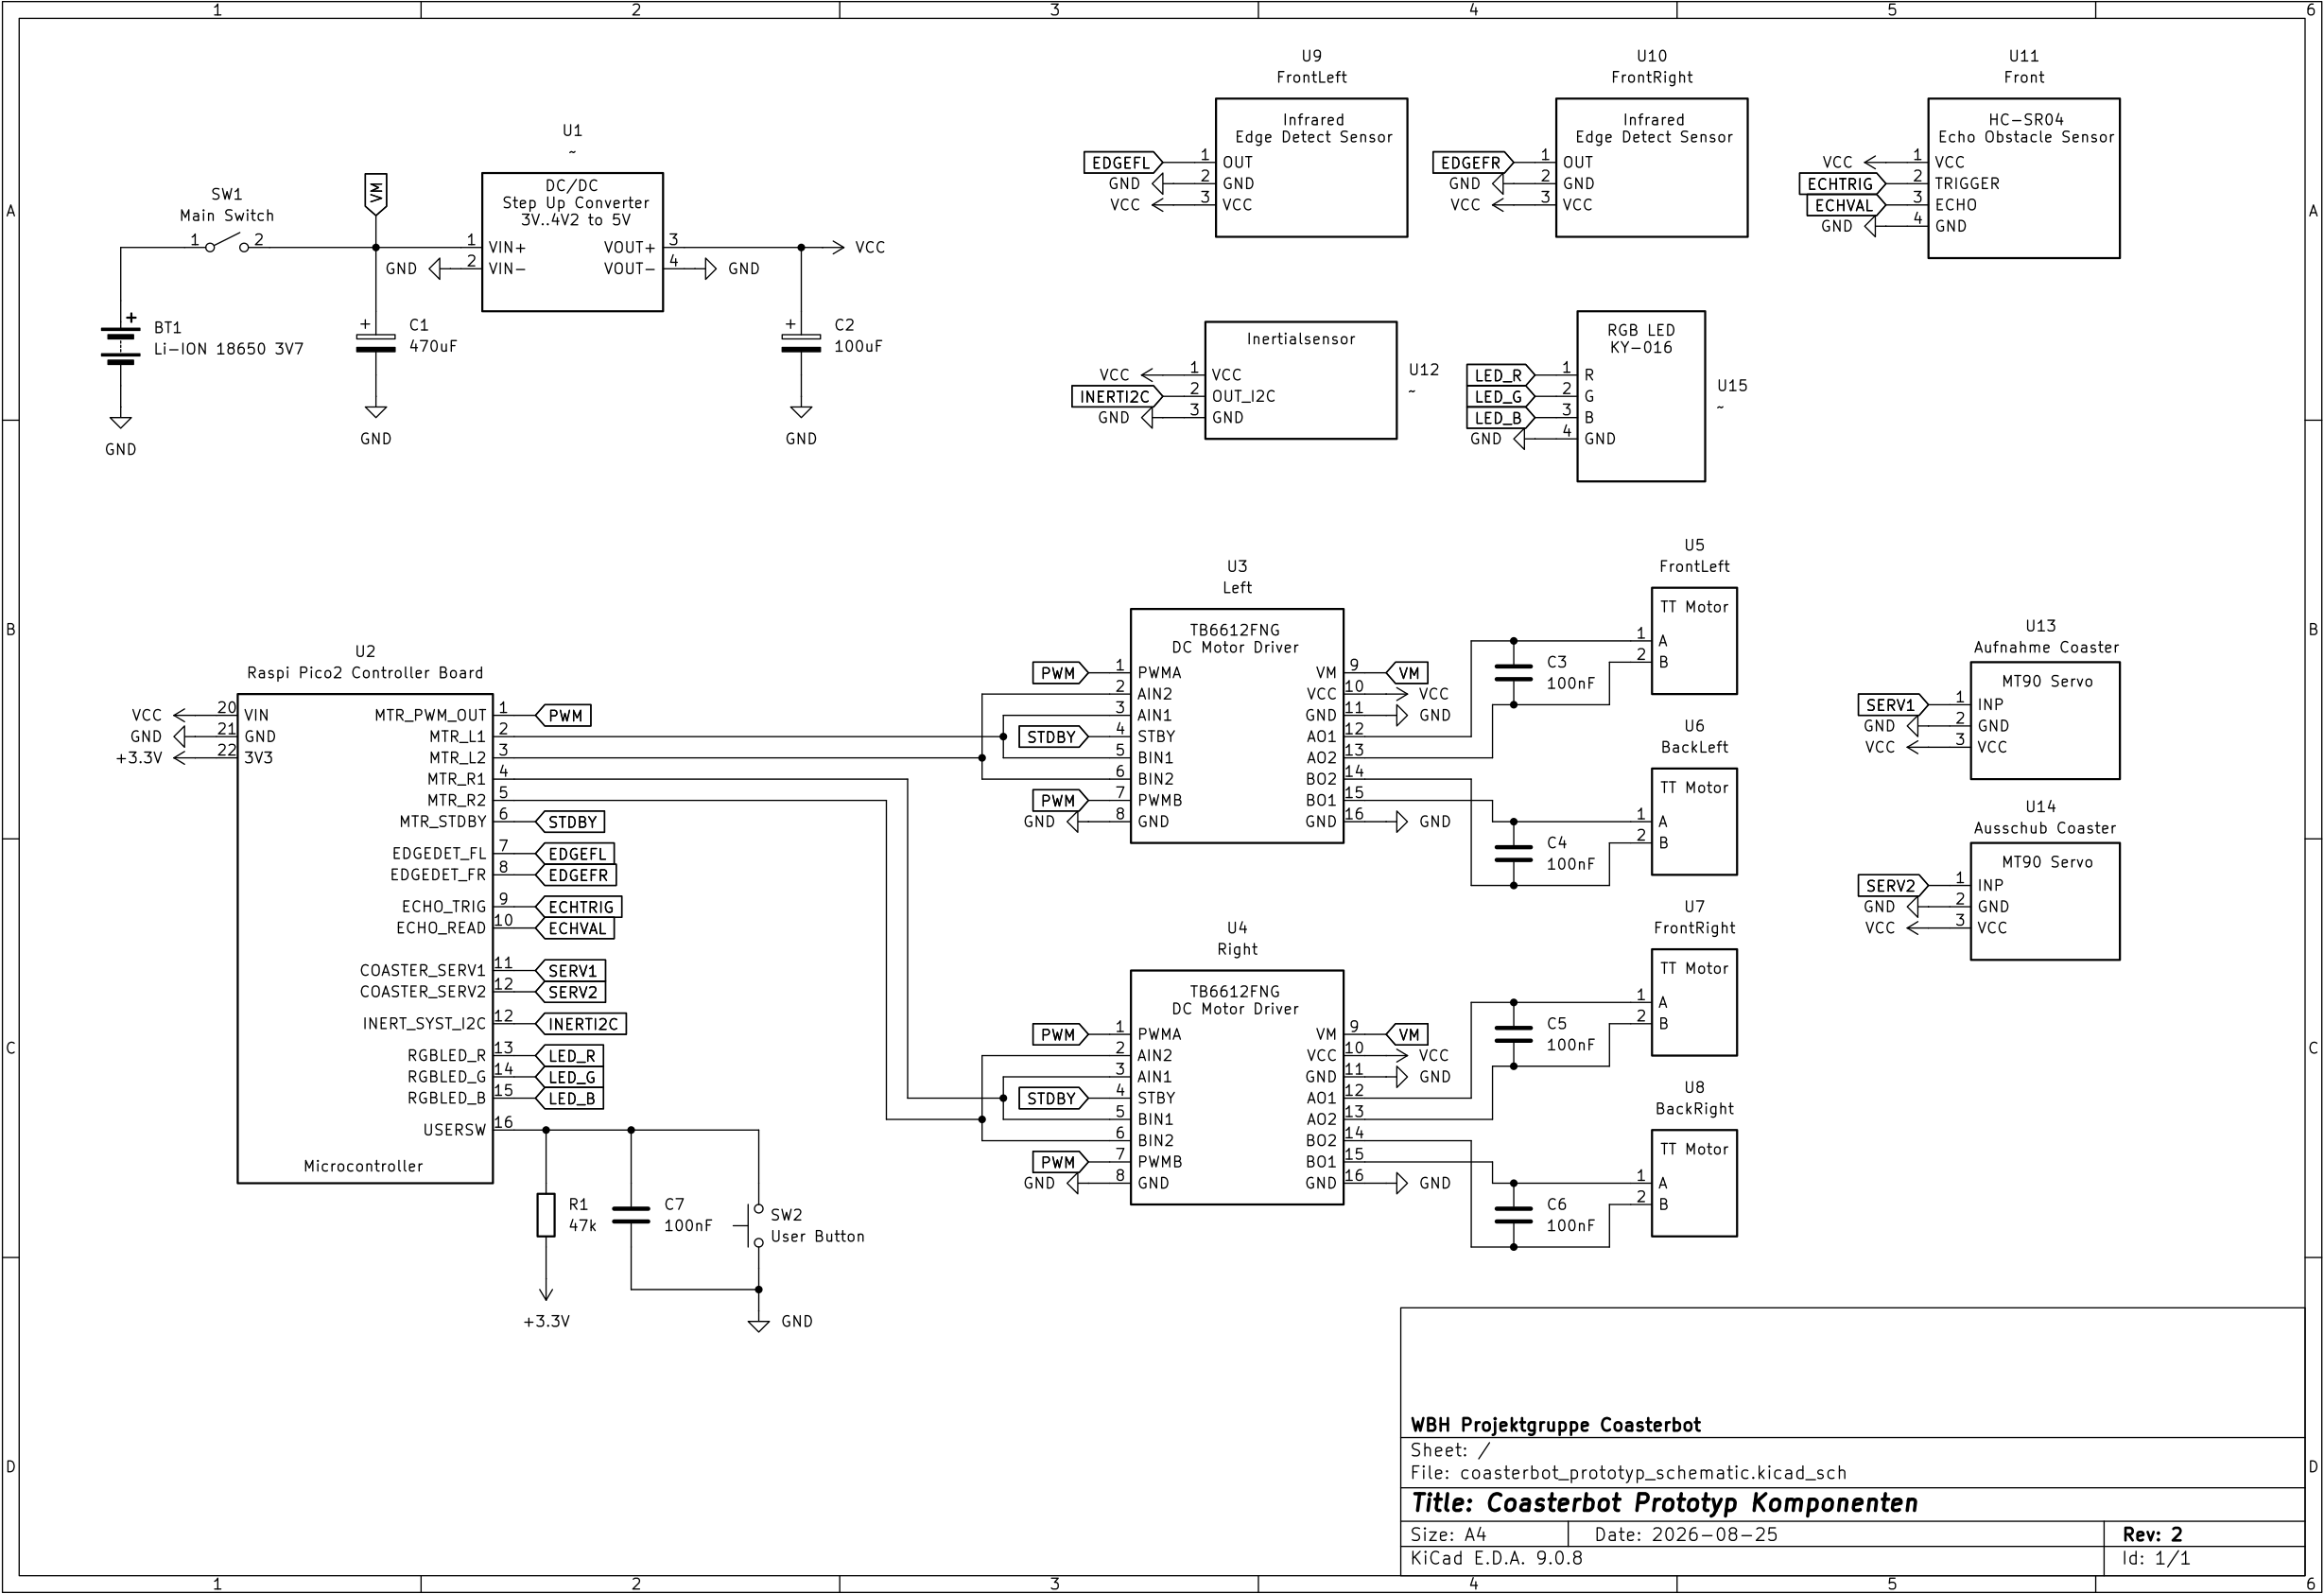
\includegraphics[width=\textwidth]{../M4_Test-und-Validierung/aufbauanleitung/schematic.png}
  \caption{Gesamtschaltung der Elektronik (aus der Aufbauanleitung).}
  \label{fig:endbericht-schematic}
\end{figure}

Beide Motoren einer Seite sind durch je einen Motortreiber geregelt, wobei sich beide Motortreiber das Standby- sowie PWM-Signal teilen. Dadurch drehen alle Motoren stets betragsmäßig gleich schnell. In der Folge sind nur Geradeausfahrt vorwärts/rückwärts als auch bei entgegengesetzter Drehrichtung Kurven auf der Stelle möglich. Diese Vereinfachung kann für eine zukünftige Ausbaustufe eventuell überdacht werden, da die Positionserkennung durch Odometrie(Zählen der Rad-Rotationen) bei Rotation auf der Stelle verhätnismßig ungenau ausfällt. Dies ergab sich in den Inbetriebnahmetests und wurde durch das Intertialsystem kompensiert. 


\subsubsection*{Hardwareabstraktion}

Die zentrale Schnittstelle ist die abstrakte C++-Klasse \texttt{RobotHAL}, die in der Simulation parallel zur Entwicklung der Elektronik definiert wurde. Sie beschreibt die Fähigkeiteiten des Roboters(Geschwindigkeit je Seite, Objektdistanz nach vorne, Kantensensor, Drehrate, Encoderwinkel, Zeit, Servosteuerung und LED), und referenziert weder die Webots Implementierung noch die eigentlichen Hardwareimplementierungen. Diese abstrakte Basisklasse wird dann in der \texttt{HardwareImplementationHAL} implementiert und bindet dann die Controller der einzelnen Komponenten ein. Diese Controller sind im Projekt Source Code als Template Klassen für die Hardwareparameter auf dem Arduino Framework implementiert. In der Hardwareabstraktion werden dann alle Controller mit den entsprechenden Pins aus einer Projektkonfigurationsdatei instanziiert und kombiniert. 

Alle Komponenten sind \textit{non-blocking} implementiert. Wenn z.B. die Motorsteuerung einer Seite sich derzeit in Vorwärtsdrehung befindet, dann durch die Steuerung aber ein Richtungswechsel ausgelöst wird, so muss zunächst aktiv abgebremst werden und erst wenn dieser Bremsvorgang beendet ist darf der Motor wieder in Rückwärtsrichtung angesteuert werden. Solche zeitabhängigen Vorgänge können natürlich durch \texttt{delay}/\texttt{sleep}-Befehle gelöst werden, in dieser Zeit erfolgt aber auch keine Sensorauswertung oder weitere Parametrierungen. Der Non-blocking Ansatz implementiert in den Komponenten jeweils eine interne Statemachine, die nach variablen Zeitintervallen einen Zustandsübergang durchführt und die Ausgangssignale anpasst oder nur in fixen Zeitintervallen Sensorwerte wiederum ausliest. Alle Aktionen finden in der Anwendungslogik weiterhin seriell statt, aber in geplanten Intervallen in \texttt{step} oder \texttt{update} Methoden, die in jedem Hauptschleifenzyklus durchlaufen werden und meistens direkt zurückspringen (Early Exit). 

\subsubsection*{Anpassungen während der Umsetzung}

Der ursprüngliche Ansatz für das Positionierungssystem war eine Integration des Beschleunigungssensors um einen Geschwindigkeitswert zu erhalten, Da die TT Motoren eine solche Information schlicht nicht bereitstellen können. Dieser Geschwindigkeitswert sollte wiederum integriert werden um eine absolute Positionierung zu erhalten. 

Während der Hardwaretests zeigte sich, dass trotz Bias-Kalibrierung, Lagekorrektur und Stillstandserkennung in Verbindung mit der Motorsteuerung die erreichbare Genauigkeit für ein Positionssystem außerhalb akzeptabler Toleranz lag: Durch Testfahrten immer wieder vorwärts und rückwärts summierte sich ein Fehler auf die aktuelle Position von einigen Dezimetern mit steigender Tendenz. In der Folge wurde die Motorhalterung modifiziert und an der dem Rad abgewandten Seite zweier TT Motoren eine Gabellichtschranke mit 20-Loch Drehscheibe und LM393 Komparator angebracht. Durch diese Kodierung ist die Änderung des Radwinkels mit $\sfrac{1}{40}$ des Umfangs bestimmbar, bei Raddurchmesser von $66$ Millimeter ergibt sich bei einem \textit{Tick} am Sensor(Wert-Wechsel) eine Fahrtstrecke von $66 \times \sfrac{\pi}{40} = 5.2$ Millimeter. Dies ist für eine gemessene Strecke zwar noch akzeptabel, aber bei Rotation wiederum zu ungenau um einen echten Drehwinkel für ein Navigationssystem zu bestimmen, weshalb der Drehwinkel weiterhin durch das IMU-System bezogen wird, wo Rotationswinkel weniger fehlerbehaftet sind als lineare Beschleunigungen. Bei der Implementierung der Tick-Erkennung wurde zusätzlich noch mit einem Hardwareinterrupt gearbeitet und konsekutive Ticks aufsummiert um sicherzustellen, dass nicht durch zu geringe Hauptschleifenfrequenz Ticks verloren gehen. Zudem wurden beide dieser Odometriecontroller mit der Motorsteuerung gekoppelt, sodass die Drehrichtung des jeweiligen Rades berücksichtigt wurde. 

Weitergehend wurde festgestellt, dass eine Drehbewegung auf der Stelle ein deutlich höheres Drehmoment im Gegensatz zu Geradeausfahrt bedarf. Dies wurde in der Motorsteuerung berücksichtigt, allerdings ist der Schlupf der Räder auf einer Tischoberfläche hier sehr hoch. Vermutlich ist also in der Folge eine Navigation mit \textit{sanften Kurven} doch zweckmäßiger. Dies sollte für eine weitere Ausbaustufe wie bereits erwähnt in Betracht gezogen werden. 

Derzeit noch nicht umgesetzt sind die Akkuüberwachung (\texttt{HW-PWR-002/003}) sowie eine Rückkopplung von Odometriesystem zu Motorsteuerung um eine tatsächliche Geschwindigkeitsregelung auf $\frac{m}{s}$ zu erreichen. Die Ansteuerung der Motoren erfolgt über das PWM Signal, das lediglich von $0$ für minimalem bis $255$ für maximales Drehmoment parametriert werden kann, die tatsächliche Drehgeschwindigkeit ist aber dann wiederum von der Motorspannung \texttt{VM} abhängig. 

